\documentclass[journal,12pt,twocolumn]{IEEEtran}
\title{Assignment 3}
\author{Varenya Upadhyaya EP20BTECH11026}
\date{}

\usepackage[utf8]{inputenc}
\usepackage{amsmath}
\usepackage{enumitem}
\usepackage{multicol}
\usepackage[english]{babel}
\usepackage{listings}
\usepackage{tabularx}
\usepackage{longtable}
\usepackage{graphicx}
\usepackage{amssymb}
\lstset{
%language=C,
frame=single, 
breaklines=true,
columns=fullflexible
}
\begin{document}

\maketitle
Download all python codes from:
\begin{lstlisting}
https://github.com/varenya27/AI1103/blob/main/Assignment3/codes
\end{lstlisting}
and all latex-tikz codes from:
\begin{lstlisting}
https://github.com/varenya27/AI1103/blob/main/Assignment3/main.tex
\end{lstlisting}
\maketitle   
\begin{center}
\section*{\textbf{Problem}}
\end{center}
Let (X,Y) be the coordinates of a point chosen at random inside the disc $x^2 + y^2 \leq r^2$ where $r\geq 0$. The probability that $Y \geq mX$ is
\begin{enumerate}[label = (\alph*)]
\begin{multicols}{2}
\setlength\itemsep{2em}
    \item $\dfrac{1}{2^r}$
    \item $\dfrac{1}{2^m}$
    \item $\dfrac{1}{2}$
    \item $\dfrac{1}{2^{r+m}}$
\end{multicols}
\end{enumerate}

\maketitle
\section*{\textbf{Solution}}
We know that the equation 
\begin{equation} 
x^2 + y^2 \leq r^2 
\end{equation}
represents a disc of radius $r$ centred at the origin, while 
\begin{equation}
y - mx \geq 0
\end{equation} represents the region above a line passing through the origin with a slope $m$. Also, the line $y=mx$ is a diameter to the circle $x^2 + y^2 = r^2$.\\
$(X,Y)$ is a point selected on the disc. Let a random variable $Z \in \{0,1\}$ represent the possible outcomes of the experiment of selecting a point on the disc.

\begin{table}[h]
\centering
    \begin{tabular}{|c|c|}
        \hline
        Equation satisfied by (X,Y)& Z    \\\hline
        $y-mx<0$ & 0    \\\hline
        $y-mx\geq0$ & 1 \\\hline
    \end{tabular}
\caption{Outcome of the Experiment}
\label{table=1}
\end{table}

Since the given line is a diameter of the circle, the number of points on either sides will be equal.
\begin{equation}
    \Rightarrow n(Z=0) = n(Z=1)
\end{equation}
The required probability can be calculated as follows:
\begin{equation}
    P(Z=1) = \frac{n(Z=1)}{n(Z=1)+n(Z=0)}
\end{equation}
\begin{equation}
    \Rightarrow P(Z=1) = \frac{1}{2}
\end{equation}
\\ $\therefore$ option (c) is correct.

\begin{figure}[!htb]
\centering
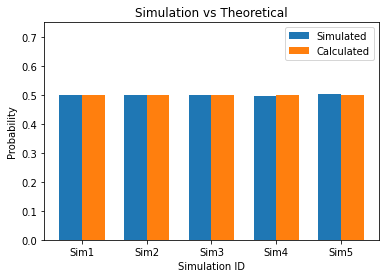
\includegraphics[width = 0.45\textwidth]{bar.png}
\label{}
\caption{Comparison between the practical and calculated values of the probability}
\end{figure}


\end{document}

